% Options for packages loaded elsewhere
\PassOptionsToPackage{unicode}{hyperref}
\PassOptionsToPackage{hyphens}{url}
%
\documentclass[
  english,
  man]{apa6}
\usepackage{lmodern}
\usepackage{amssymb,amsmath}
\usepackage{ifxetex,ifluatex}
\ifnum 0\ifxetex 1\fi\ifluatex 1\fi=0 % if pdftex
  \usepackage[T1]{fontenc}
  \usepackage[utf8]{inputenc}
  \usepackage{textcomp} % provide euro and other symbols
\else % if luatex or xetex
  \usepackage{unicode-math}
  \defaultfontfeatures{Scale=MatchLowercase}
  \defaultfontfeatures[\rmfamily]{Ligatures=TeX,Scale=1}
\fi
% Use upquote if available, for straight quotes in verbatim environments
\IfFileExists{upquote.sty}{\usepackage{upquote}}{}
\IfFileExists{microtype.sty}{% use microtype if available
  \usepackage[]{microtype}
  \UseMicrotypeSet[protrusion]{basicmath} % disable protrusion for tt fonts
}{}
\makeatletter
\@ifundefined{KOMAClassName}{% if non-KOMA class
  \IfFileExists{parskip.sty}{%
    \usepackage{parskip}
  }{% else
    \setlength{\parindent}{0pt}
    \setlength{\parskip}{6pt plus 2pt minus 1pt}}
}{% if KOMA class
  \KOMAoptions{parskip=half}}
\makeatother
\usepackage{xcolor}
\IfFileExists{xurl.sty}{\usepackage{xurl}}{} % add URL line breaks if available
\IfFileExists{bookmark.sty}{\usepackage{bookmark}}{\usepackage{hyperref}}
\hypersetup{
  pdftitle={Bail Setting Patterns in New York City},
  pdfauthor={Jeff Shamp1},
  pdflang={en-EN},
  pdfkeywords={bail, reform, pretrial detention, Rikers, cash bail},
  hidelinks,
  pdfcreator={LaTeX via pandoc}}
\urlstyle{same} % disable monospaced font for URLs
\usepackage{color}
\usepackage{fancyvrb}
\newcommand{\VerbBar}{|}
\newcommand{\VERB}{\Verb[commandchars=\\\{\}]}
\DefineVerbatimEnvironment{Highlighting}{Verbatim}{commandchars=\\\{\}}
% Add ',fontsize=\small' for more characters per line
\usepackage{framed}
\definecolor{shadecolor}{RGB}{248,248,248}
\newenvironment{Shaded}{\begin{snugshade}}{\end{snugshade}}
\newcommand{\AlertTok}[1]{\textcolor[rgb]{0.94,0.16,0.16}{#1}}
\newcommand{\AnnotationTok}[1]{\textcolor[rgb]{0.56,0.35,0.01}{\textbf{\textit{#1}}}}
\newcommand{\AttributeTok}[1]{\textcolor[rgb]{0.77,0.63,0.00}{#1}}
\newcommand{\BaseNTok}[1]{\textcolor[rgb]{0.00,0.00,0.81}{#1}}
\newcommand{\BuiltInTok}[1]{#1}
\newcommand{\CharTok}[1]{\textcolor[rgb]{0.31,0.60,0.02}{#1}}
\newcommand{\CommentTok}[1]{\textcolor[rgb]{0.56,0.35,0.01}{\textit{#1}}}
\newcommand{\CommentVarTok}[1]{\textcolor[rgb]{0.56,0.35,0.01}{\textbf{\textit{#1}}}}
\newcommand{\ConstantTok}[1]{\textcolor[rgb]{0.00,0.00,0.00}{#1}}
\newcommand{\ControlFlowTok}[1]{\textcolor[rgb]{0.13,0.29,0.53}{\textbf{#1}}}
\newcommand{\DataTypeTok}[1]{\textcolor[rgb]{0.13,0.29,0.53}{#1}}
\newcommand{\DecValTok}[1]{\textcolor[rgb]{0.00,0.00,0.81}{#1}}
\newcommand{\DocumentationTok}[1]{\textcolor[rgb]{0.56,0.35,0.01}{\textbf{\textit{#1}}}}
\newcommand{\ErrorTok}[1]{\textcolor[rgb]{0.64,0.00,0.00}{\textbf{#1}}}
\newcommand{\ExtensionTok}[1]{#1}
\newcommand{\FloatTok}[1]{\textcolor[rgb]{0.00,0.00,0.81}{#1}}
\newcommand{\FunctionTok}[1]{\textcolor[rgb]{0.00,0.00,0.00}{#1}}
\newcommand{\ImportTok}[1]{#1}
\newcommand{\InformationTok}[1]{\textcolor[rgb]{0.56,0.35,0.01}{\textbf{\textit{#1}}}}
\newcommand{\KeywordTok}[1]{\textcolor[rgb]{0.13,0.29,0.53}{\textbf{#1}}}
\newcommand{\NormalTok}[1]{#1}
\newcommand{\OperatorTok}[1]{\textcolor[rgb]{0.81,0.36,0.00}{\textbf{#1}}}
\newcommand{\OtherTok}[1]{\textcolor[rgb]{0.56,0.35,0.01}{#1}}
\newcommand{\PreprocessorTok}[1]{\textcolor[rgb]{0.56,0.35,0.01}{\textit{#1}}}
\newcommand{\RegionMarkerTok}[1]{#1}
\newcommand{\SpecialCharTok}[1]{\textcolor[rgb]{0.00,0.00,0.00}{#1}}
\newcommand{\SpecialStringTok}[1]{\textcolor[rgb]{0.31,0.60,0.02}{#1}}
\newcommand{\StringTok}[1]{\textcolor[rgb]{0.31,0.60,0.02}{#1}}
\newcommand{\VariableTok}[1]{\textcolor[rgb]{0.00,0.00,0.00}{#1}}
\newcommand{\VerbatimStringTok}[1]{\textcolor[rgb]{0.31,0.60,0.02}{#1}}
\newcommand{\WarningTok}[1]{\textcolor[rgb]{0.56,0.35,0.01}{\textbf{\textit{#1}}}}
\usepackage{graphicx,grffile}
\makeatletter
\def\maxwidth{\ifdim\Gin@nat@width>\linewidth\linewidth\else\Gin@nat@width\fi}
\def\maxheight{\ifdim\Gin@nat@height>\textheight\textheight\else\Gin@nat@height\fi}
\makeatother
% Scale images if necessary, so that they will not overflow the page
% margins by default, and it is still possible to overwrite the defaults
% using explicit options in \includegraphics[width, height, ...]{}
\setkeys{Gin}{width=\maxwidth,height=\maxheight,keepaspectratio}
% Set default figure placement to htbp
\makeatletter
\def\fps@figure{htbp}
\makeatother
\setlength{\emergencystretch}{3em} % prevent overfull lines
\providecommand{\tightlist}{%
  \setlength{\itemsep}{0pt}\setlength{\parskip}{0pt}}
\setcounter{secnumdepth}{-\maxdimen} % remove section numbering
% Make \paragraph and \subparagraph free-standing
\ifx\paragraph\undefined\else
  \let\oldparagraph\paragraph
  \renewcommand{\paragraph}[1]{\oldparagraph{#1}\mbox{}}
\fi
\ifx\subparagraph\undefined\else
  \let\oldsubparagraph\subparagraph
  \renewcommand{\subparagraph}[1]{\oldsubparagraph{#1}\mbox{}}
\fi
% Manuscript styling
\usepackage{upgreek}
\captionsetup{font=singlespacing,justification=justified}

% Table formatting
\usepackage{longtable}
\usepackage{lscape}
% \usepackage[counterclockwise]{rotating}   % Landscape page setup for large tables
\usepackage{multirow}		% Table styling
\usepackage{tabularx}		% Control Column width
\usepackage[flushleft]{threeparttable}	% Allows for three part tables with a specified notes section
\usepackage{threeparttablex}            % Lets threeparttable work with longtable

% Create new environments so endfloat can handle them
% \newenvironment{ltable}
%   {\begin{landscape}\centering\begin{threeparttable}}
%   {\end{threeparttable}\end{landscape}}
\newenvironment{lltable}{\begin{landscape}\centering\begin{ThreePartTable}}{\end{ThreePartTable}\end{landscape}}

% Enables adjusting longtable caption width to table width
% Solution found at http://golatex.de/longtable-mit-caption-so-breit-wie-die-tabelle-t15767.html
\makeatletter
\newcommand\LastLTentrywidth{1em}
\newlength\longtablewidth
\setlength{\longtablewidth}{1in}
\newcommand{\getlongtablewidth}{\begingroup \ifcsname LT@\roman{LT@tables}\endcsname \global\longtablewidth=0pt \renewcommand{\LT@entry}[2]{\global\advance\longtablewidth by ##2\relax\gdef\LastLTentrywidth{##2}}\@nameuse{LT@\roman{LT@tables}} \fi \endgroup}

% \setlength{\parindent}{0.5in}
% \setlength{\parskip}{0pt plus 0pt minus 0pt}

% \usepackage{etoolbox}
\makeatletter
\patchcmd{\HyOrg@maketitle}
  {\section{\normalfont\normalsize\abstractname}}
  {\section*{\normalfont\normalsize\abstractname}}
  {}{\typeout{Failed to patch abstract.}}
\patchcmd{\HyOrg@maketitle}
  {\section{\protect\normalfont{\@title}}}
  {\section*{\protect\normalfont{\@title}}}
  {}{\typeout{Failed to patch title.}}
\makeatother
\shorttitle{Bail Reform Review}
\keywords{bail, reform, pretrial detention, Rikers, cash bail\newline\indent Word count: 3446}
\DeclareDelayedFloatFlavor{ThreePartTable}{table}
\DeclareDelayedFloatFlavor{lltable}{table}
\DeclareDelayedFloatFlavor*{longtable}{table}
\makeatletter
\renewcommand{\efloat@iwrite}[1]{\immediate\expandafter\protected@write\csname efloat@post#1\endcsname{}}
\makeatother
\usepackage{csquotes}
\ifxetex
  % Load polyglossia as late as possible: uses bidi with RTL langages (e.g. Hebrew, Arabic)
  \usepackage{polyglossia}
  \setmainlanguage[]{english}
\else
  \usepackage[shorthands=off,main=english]{babel}
\fi

\title{Bail Setting Patterns in New York City}
\author{Jeff Shamp\textsuperscript{1}}
\date{}


\authornote{

Masters capstone project for The City University of New York, School of Professional Studies. This is an extension of the work I began while at the Bronx Defenders regarding the effectiveness of recent (2020) bail reform in the state of the New York.

Correspondence concerning this article should be addressed to Jeff Shamp, 22 Irving Place, New York. E-mail: \href{mailto:shamp.jeff@gmail.com}{\nolinkurl{shamp.jeff@gmail.com}}

}

\affiliation{\vspace{0.5cm}\textsuperscript{1} CUNY SPS - MSDS}

\abstract{
Recent reforms to the bail system were implemented in the state of the New York in 2020. The intent of the reforms was to reduce the number of people incarcerated pretrial by allowing reduced cash bail, adding multiple payment options, and reducing the number of offenses that are bail eligible. The vast majority of people in local jails were unable post bail. This has led to surging jail populations, unsafe conditions for inmates and staff, and downstream effects on families who may rely on the incarcerated person for financial or social needs. Many individuals detained pretrial are charged with non-violent crimes and pose no serious ``flight risk''. The reforms still maintained a high level of discretion for judges to set bail and offered no strict guidelines for determining bail amounts, only that judges should ``consider the financial situation'' of the defendant in setting bail. Judges appear to be ignoring the law's requirement to consider the financial status of the defendant and are simply setting bail similarly to how they have previously. We show that, in general, judges have not meaningfully changed their bail setting practices and rarely consider the unique financial situation of the defendant. This is result is somewhat expected as previous research has demonstrated this effect in other states. Bail setting patterns in New York City only briefly changed immediately after the reforms were enacted, and have since resumed their historical values for many crime categories. This has, in part, led to the rising prison population on Riker's Island and the deterioration of the safety at the facility. Pretrial detention continues to be the primary reason for incarceration at Riker's Island due to the failure to meaningfully reduce the barriers to posting bail or release on recognizance.
}



\begin{document}
\maketitle

\hypertarget{introduction}{%
\section{Introduction}\label{introduction}}

\hypertarget{participant}{%
\subsection{Participant}\label{participant}}

\emph{Jeff Shamp}: Jeff is the sole contributor to this document. He wrote the code to gather, clean, organize and analyze the data from the New York State Office of Court Administration. He also built the \href{https://shamp-jeff.shinyapps.io/Bail_Setting_Patterns_in_New_York_City/}{shiny app to visualize the results}.

\hypertarget{problem}{%
\subsection{Problem}\label{problem}}

Bail reform laws enacted in 2020 were meant to address the rising population of local jails, and in specifically, Riker's Island in New York City. The population of local jails is overwhelmingly the result of pretrial detention. People charged with crimes who cannot make bail are sent to jail while they await trial. Judges who set bail in criminal cases are meant to, under new laws, consider the specific financial situation of the defendant when setting bail. Additionally, several payment options must be available to defendants. If this is the case, we should see a wide diversity of bail amounts for given charges. The best case scenario would a random distribution of bail values to match the diversity of financial means present in the city of New York. We should also see a diversity of bail payments made through alternative methods (surety, credit card, bond, cash). Furthermore, bail values should not be centered around large, whole number values such as \(\$10,000\), \(\$7500\), \(\$25,000\), etc. as was common before the bail reform went into place.

\hypertarget{literature-review}{%
\section{Literature Review}\label{literature-review}}

The exploding population of inmates in the New York City jails, and commensurate violence and unsafe conditions that population has created demonstrate the need for the city to reduce the population of incarcerated people. One simple way to reduce jail populations in New York City is to reduce the number of people who are detained pretrial, especially considering that pretrial detention is, by definition, incarcerating people before they have been convicted of a crime. Limiting the number of pretrial detentions would have significant impact on the population of city jails. Nearly two-thirds of all inmates in local jails across the United States are incarcerated pretrial (Minton \& Zeng 2015) . Pretrial incarceration has huge fiscal costs. The estimated cost of detaining people pretrial across the United States is \$14 billion, approximately 17\% of total spending on corrections nationally (Gupta, et al 2016). For the individual involved, pretrial detention can have major impacts on employment, childcare, and housing (Manudeep 2018) and (Heaton, et al 2017). Additionally, much research has been conducted recently exploring the effects of pretrial detention on the defendants chance of being convicted (Stevenson 2018) as well as the length of their prison sentence (Dobbie, et al 2018). It should be noted that these downstream effects of pretrial detention result in more defendants taking guilty pleas for charges that might otherwise be dropped. Furthermore, recent research suggests that pretrial detention may increase future criminal activity (Stevenson 2015). This effect may be due to the destabilizing effect incarceration has on the life of the individual or due to pushing individuals closer to existing criminal networks (Stevenson 2015). Lastly, research suggests that current bail setting practice have disproportionate impact on people of color, which only adds importance to the need to reform (Arnold et al, 2018).

These realities have pushed some localities to reform their bail setting practices. Research suggests a fine ability to predict existing bail setting patterns in local areas (Kleinberg 2018). Kleinberg (2018) determined that both crime reduction and jail depopulation where possible if judges had access to better tools for scoring defendant release risk. However, it appears to be the case that when judges are given such tools for scoring defendant recidivism, judges are tend to ignore those inputs in lieu of their historical bail setting patterns or personal bias (Albright, 2019). It stands to reason that the discretionary system for setting bail may be the next area of reform. Having mathematical tools for determining risk are ineffective if arraignment judges ignore the results.

New York State implemented bail reform laws in 2020, but quickly rolled them back after premature pressure over perceived public safety concerns. As a result, New York has a mixed system of bail where some charges (mostly misdemeanors) are no longer eligible for bail, but some charges are still eligible. Further, under the new law, judges are to examine the individual financial state of the defendant in determining bail so as to limit excessively high bail costs. This individual stipulation is was meant to address the findings of above research, and serves an interesting marker for this paper. If judges are following the intent of the law, they should be tailoring the bail to each defendants financial situation. We suggest that this should create distribution of bail amounts that approach a random distribution. We suspect that bail amounts will not be purely randomly distributed, but should be not resemble other well-known distributions either. Additionally, we should not see disparities in bail amounts for similar charges based on race as bail setting should only reflect financial conditions. Lastly, we are additionally interested the potential effect that reform recency has on bail setting patterns. Attorneys working in the New York City courts system have anecdotal observations that bail amount vary based on how present and persistent bail reform is in public discourse (news, protests, research, etc.). If this is the case, we should see some significant deviations in bail setting practices as a function of time.

\hypertarget{methodology}{%
\section{Methodology}\label{methodology}}

Litigation for the release of pretrial data was settled by judgment in July, 2020 allowing for the release of all New York state pretrial data. This data is maintained and published by the New York Office of Court Administration and is publicly viewable at this \href{https://ww2.nycourts.gov/pretrial-release-data-33136}{web address}. The data dictionary, detailing the collected data fields is located at the following \href{https://www.nycourts.gov/legacypdfs/court-research/PretrialReleaseDataDictionaryWeb.pdf}{web adddress}. We developed custom python scripts for automatic scraping, cleaning, and organizing the data. Once the data was prepared, we were able to visual the bail setting practices in the counties that make up the city of New York. We primarily focused on the following questions regarding bail.

\begin{enumerate}
\def\labelenumi{\arabic{enumi}.}
\tightlist
\item
  Are bail amounts centered on large, whole number values or disperse to reflect the financial situation of the defendant?
\item
  To what extent are bail values impacted by race or ethnicity?
\item
  Is bail impacted by judges who regularly work in New York City, or less common judges?
\item
  Are there specific judges that consistently set higher or lower bail amount?
\end{enumerate}

We compiled our analysis into an interactive dashboard where advocates, lawyers, and the concerned public could view the bail setting patterns in New York City by specific charge as well as by specific judges.

For this analysis, we focused on cash bail amounts. This is due to the fact that cash bail is very common and the average cash bail is the same as the average bail bond amount. Part of the reform laws was to ensure a diversity of bail types, however for many very low income people, any amount is unattainable. There is conjecture as to whether judges are thwarting the reform laws by setting significantly higher bail amounts for \enquote{easier} payment options like surety bonds, but we will leave that to future work. It should be noted that we disregarded the \enquote{dollar bail} values contained within the data set. Bail values set to single digit values, usually \(\$1\), are set concurrently with bail for other charges. For example, if a defendant is charged with one alleged crime and bail is set for \(\$10,000\) and also charged separately with another alleged crime, then the second bail is set at one dollar. This can go on for several allegations leading to several \enquote{dollar} bails. To avoid this situation skewing the bail setting practices, we omitted bail values under ten dollars.

It should be noted that the original law exempted a large section of misdemeanor offenses from bail, but after June 1, 2020 some of those misdemeanor offenses were bail eligible. That inclusion of bail eligibility may skew the distribution of some arraignment charges.

\hypertarget{results}{%
\section{Results}\label{results}}

The data set contained all criminal arraignments in New York City for the calendar year 2020 and contains 11,808 cases. In this time period, bail reform was implemented starting January 1, 2020 and ran in full effect until June 1, 2020 when the laws were amended due to political pressure. While, it would be best to see a full year of implementation, it is good to be able to compare the full effect of the law to scaled back version in the same data set.

To view and further explore this data set, \href{https://shamp-jeff.shinyapps.io/Bail_Setting_Patterns_in_New_York_City/}{see this interactive visualization}

\hypertarget{bail-amounts-by-payment-type}{%
\subsection{Bail Amounts by Payment Type}\label{bail-amounts-by-payment-type}}

Part of the reform laws was to require a diversity of payment options, e.g.~bond company, credit card, cash, or surety bond, but the traditional cash and bail bond payment methods continue to be the primary form of posting bail.

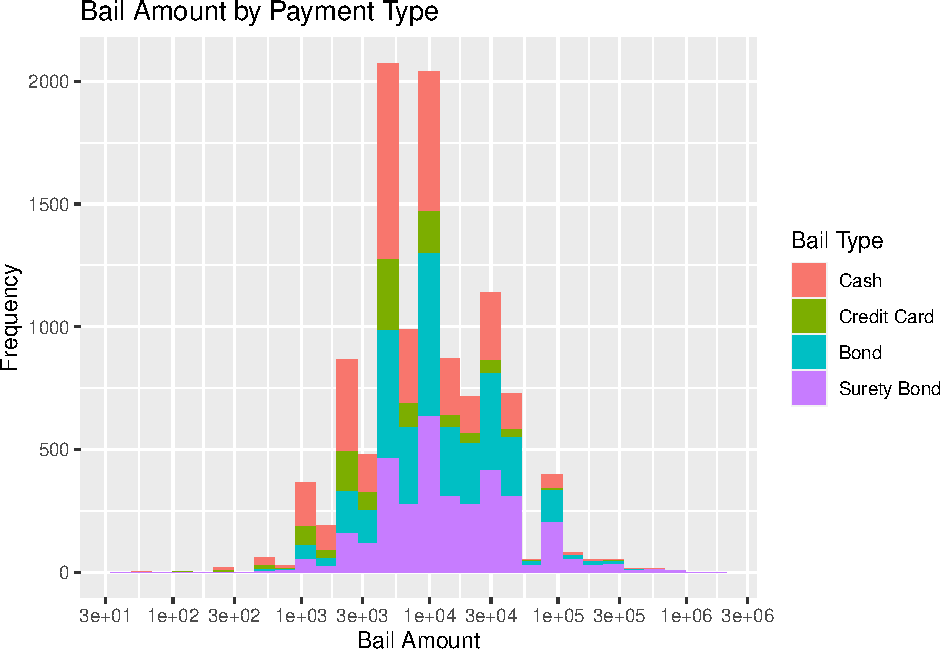
\includegraphics{bail_reform_shamp_thesis_files/figure-latex/bail_amount_payment-1.pdf}

Here we see a roughly normal distribution of bail amounts by payment type, we also see that bail amounts are most often occurring at large whole number values like \(\$5000\), \(\$10000\), and \(\$30000\). According to advocates who helped shaped the reform laws, this pile up at whole number values should not be happening. We will more closely examine how these bail values change over the course of 2020 and by specific charge.

\hypertarget{cash-bail-by-common-charges}{%
\subsection{Cash Bail by Common Charges}\label{cash-bail-by-common-charges}}

\begin{table}[h]

\begin{center}
\begin{threeparttable}

\caption{\label{tab:most_common_charges}Frequency of Bail Eligible Charges}

\begin{tabular}{ll}
\toprule
top\_charge\_at\_arraign & \multicolumn{1}{c}{count\_charge}\\
\midrule
pl 265.03 03 cf cpw-2nd: loaded firearm & 1319\\
pl 120.05 02 df aslt w/int cause ph inj w/weap & 628\\
pl 120.00 01 am aslt 3-w/int cause phys injury & 583\\
pl 265.03 01b cf cpw-2nd: loaded firearm & 555\\
pl 140.25 02 cf burglary 2nd- dwelling & 463\\
\bottomrule
\end{tabular}

\end{threeparttable}
\end{center}

\end{table}

Given these common charges in Table 1 we will examine a few bail amount distributions over the course of the year. These distributions should have a wide distribution and should not center around whole number values. The literature suggests that bail values tend to change drastically once reforms are implemented, then tend to return to previous historical values where judges have discretion to set bail amounts.

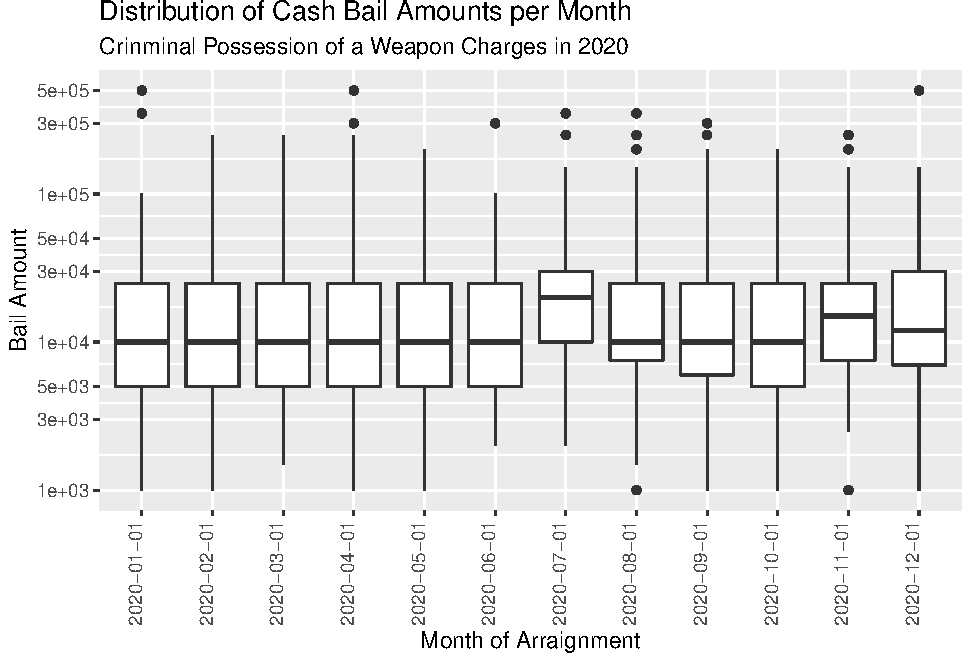
\includegraphics{bail_reform_shamp_thesis_files/figure-latex/charge_distrb_cpw-1.pdf}

For the most common charge in the state of New York, criminal possession of a firearm we see a normal distribution of cash bail amounts month over month. The only notable exception is in July, right after the reform rollback took place. In July we see a large spike in bail amounts from a median value of roughly \(\$10,000\) to nearly \(\$30,000\) median bail amount. This figure suggests that judges are not tailoring bail to defendants financial situations, they are simply posting bail at some previously decided high value, and their discretion to set bail can result in higher values whenever they see fit. None of the above points are in keeping with the bail reform laws passed by the legislature.

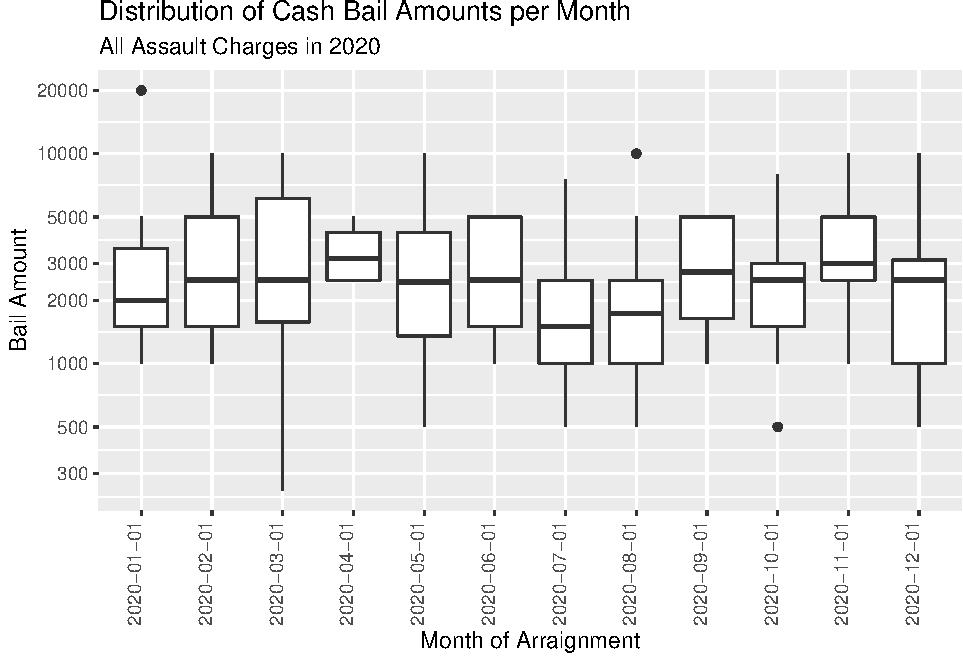
\includegraphics{bail_reform_shamp_thesis_files/figure-latex/charge_distrb_120-1.pdf}

For all assault category charges in 2020 we see more variance in the cash bail amounts. During the January 1, 2020 through June 1, 2020 full reform period the median bail value was between \(\$2,000\) to \(\$3,000\), with right tails into higher values. Outliers for assault charges started at \(\$10,000\). After the roll back in reform laws, the period after July 1, 2020, we see a similar effect as found in the literature review. Bail values dropped significantly to a median value between \(\$1,000 - \$2,000\) for a couple of months only to resume the typical \(\$2,000\) to \(\$3,000\) median value range.

\hypertarget{distribution-by-race-and-ethnicity}{%
\subsubsection{Distribution by Race and Ethnicity}\label{distribution-by-race-and-ethnicity}}

We also examined to what extent race and ethnicity may impact the bail setting patterns of judges in New York City. Again, we will focus on some common charges to ensure that we have adequate data.

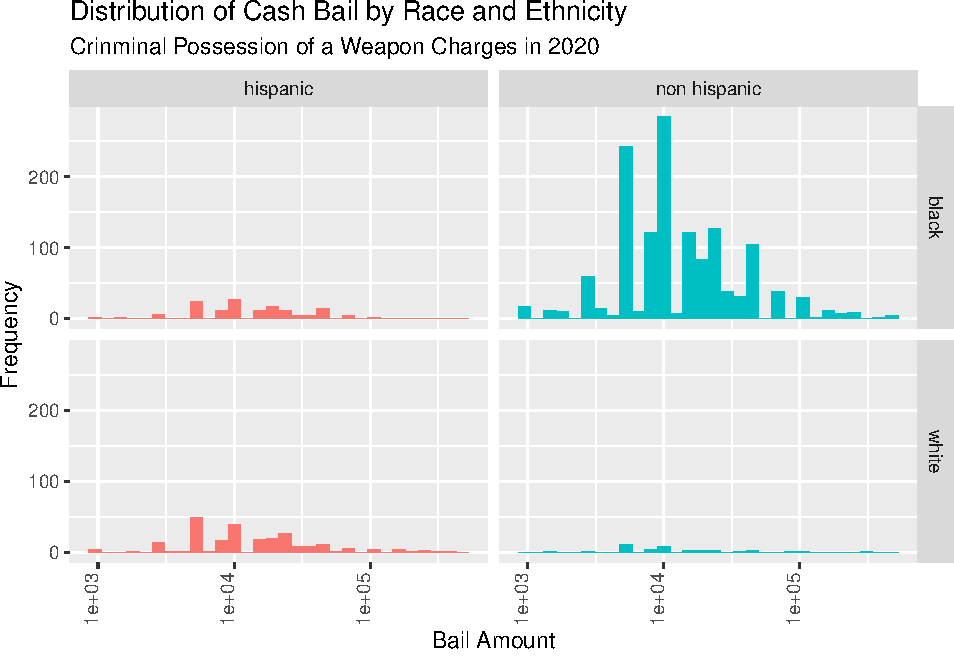
\includegraphics{bail_reform_shamp_thesis_files/figure-latex/cpw_race_distrb-1.pdf}

Other than the glaring disparity in race for who is charged with the criminal possession of a firearm, the bail values by race and ethnicity appear to be similarly bounded and normally distributed across demographics. Interesting enough, the particular charge examined above will likely be struck down by the Supreme Court this year. This will mostly like happen on second amendment grounds, but advocates for criminal justice reform also support the repeal of this law due to its incredibly disproportionate enforcement on African-Americans as shown above.

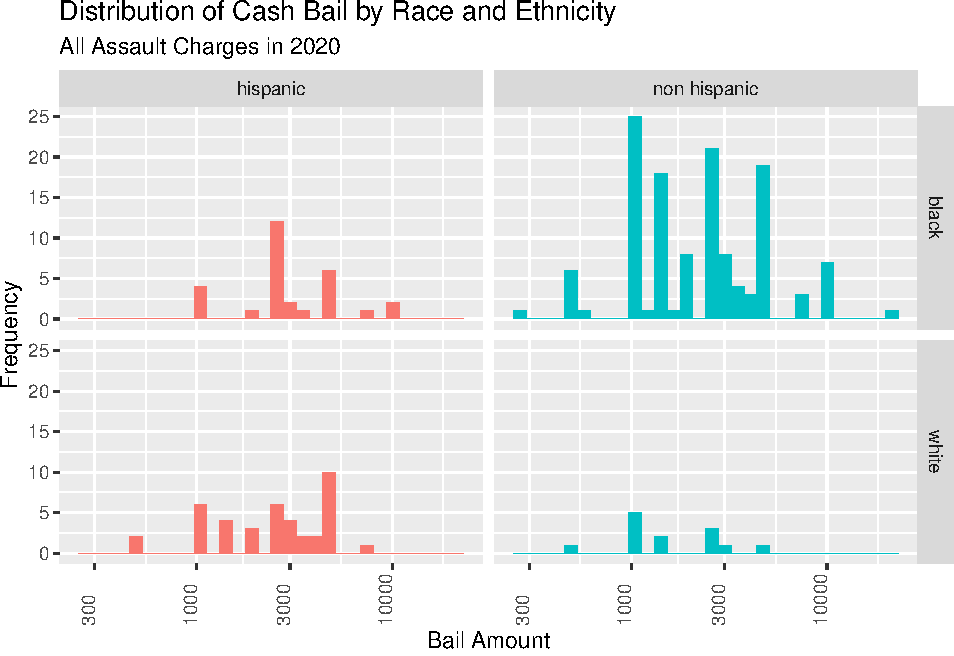
\includegraphics{bail_reform_shamp_thesis_files/figure-latex/120_race_distrb-1.pdf}

Again, we see a similar distribution of bail values across race and ethnic lines, which is a good thing. Upon investigating several specific charges, we see that this effect holds true. Judges are not using their discretion to skew higher bail values for certain demographics of people.

\hypertarget{bail-values-by-judge-frequency}{%
\subsection{Bail Values by Judge Frequency}\label{bail-values-by-judge-frequency}}

There are many judges that work in the five boroughs of the New York City and a large cross section of them are more prolific that others. This could be due to a cross section of the judges coming into New York to fill gaps in staffing or phasing out due to retirement. We want to examine the extent to which more or less common judges set different bail amounts for similar charges. We filter more common judges as those who arraign more than one hundred cases and less common judges as those who arraign less than one hundred. The one hundred case marker is median value of judge case number histogram.

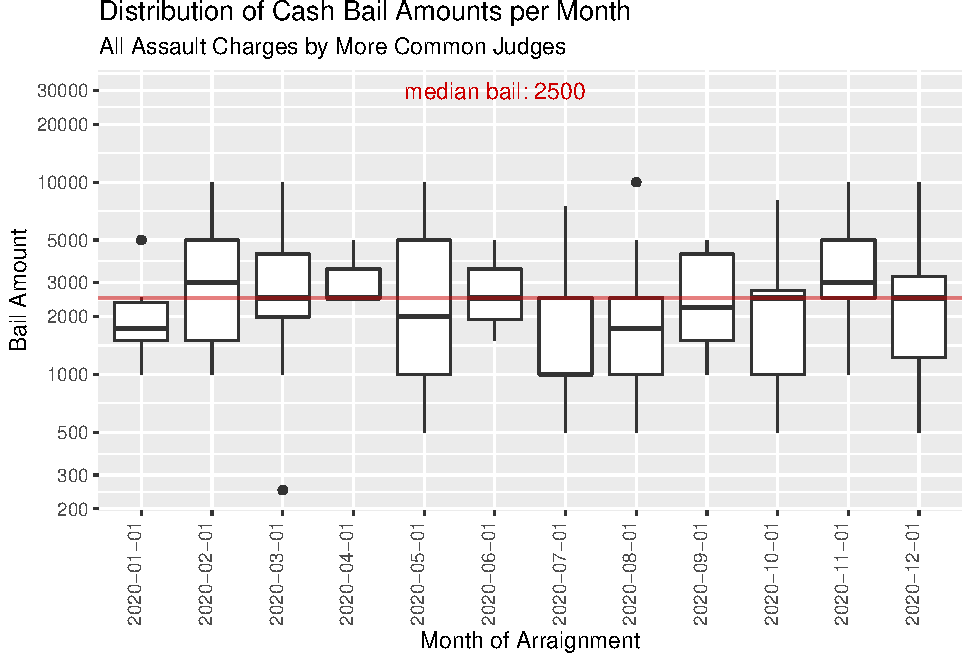
\includegraphics{bail_reform_shamp_thesis_files/figure-latex/more_less_judge-1.pdf} 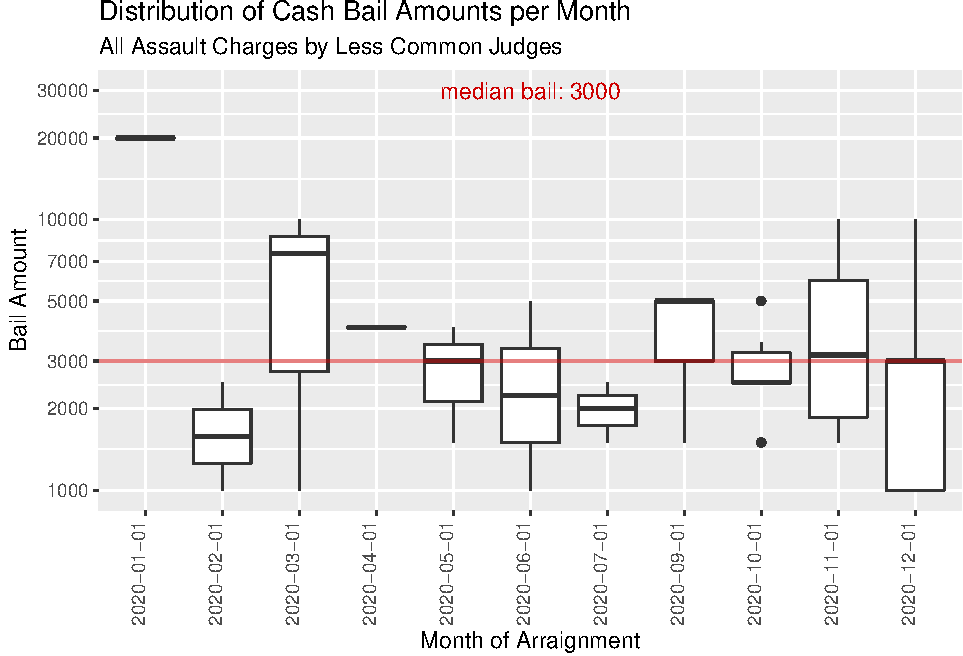
\includegraphics{bail_reform_shamp_thesis_files/figure-latex/more_less_judge-2.pdf}

For assault charges we see little difference in overall bail setting amounts on a per month bases. The median value overall for more common judges is lower when compared to less common judges. It appears to be generally true for most charges that more common and less common judges are still reasonably well-aligned in bail setting practices.

\hypertarget{discussion}{%
\section{Discussion}\label{discussion}}

\hypertarget{conclusion}{%
\subsection{Conclusion}\label{conclusion}}

The reform laws set into place in 2020 required multiple avenues for defendants to post bail. The laws also required judges to take the unique financial circumstances of the defendant into consideration in setting bail. This should imply a more random distribution of bail values depending on the financial means of the defendant. We see three things from this analysis: 1) judges are setting reasonably consistent bail amounts across several payment methods, 2) judges are setting bail amounts in a similar manner across racial and ethnic lines and, 3) judges do not appear to be considering the unique financial situation of the defendant, but rather simply using some arbitrary or historical bail value given the top charge at arraignment. This effect is consistent with the literature in that when judges are given discretion in bail setting, they often set some large whole number value that they, for any reason, decide is fair. This is, to be clear, not in keeping with the spirit of the law, but when judges are given discretion, this effect is a well-documented result.

Ideally, if the law were more tightly followed, then we should see a wider distribution of bail values set for specific charges. At the very least, we should see a left-tail shew to the distributions that shifts towards lower values. What we see consistently in this data set are clear normal distributions of bail amounts centered on some large, whole number value.

If judges cannot or will not take the financial situation of defendants into account when setting bail, and the inability for defendants to post bail causes large scale downstream consequences for the defendant, their family, and causes serious strain on local prisons e.g.~overcrowding, then judicial discretion should be minimized. Previous research as been done (Manudeep, 2018) and (Kleinberg, 2018) on how to best predict and minimize bail values based on various risk factors. We also see from Albright (2018) that having computer predicted tool and judicial discretion will likely not help reduce bail values or meaningfully improve bail setting practices.

\hypertarget{future-work}{%
\subsection{Future Work}\label{future-work}}

In light of the above bail setting practices and body of research surrounding bail setting practices nation-wide, developing a New York City specific bail setting prediction model would be helpful in replacing the current system. It would be very helpful to collect some level of financial data on defendants to assist in determining an appropriate bail in relation to the charge. That is a large undertaking at a legislative level, but we are to minimize the number of pretrial detainees by more accurately predicting appropriate bail, that would be more helpful than allowing judges to arbitrarily decide on a dollar value.

\newpage

\hypertarget{references}{%
\section{References}\label{references}}

\begingroup
\setlength{\parindent}{-0.5in}
\setlength{\leftskip}{0.5in}

Albright, A. (2019). If you give a judge a risk score: evidence from Kentucky bail decisions, Harvard John M. Olin Fellow's Discussion Paper 85.

Arnold, D \& Dobbie, W, \& Yang, C. (2018). Racial Bias in Bail Decisions,
The Quarterly Journal of Economics, Volume 133, Issue 4, Pages 1885--1932,
\url{https://doi.org/10.1093/qje/qjy012}

Bayer, P., et al., (2019). Building Criminal Capital Behind Bars: Peer Effects in Juvenile Corrections,
The Quarterly Journal of Economics 105, 105.

Dobbie, W \& Goldin, J \& Yang, C. (2018). The Effects of Pretrial Detention on Conviction, Future Crime, and Employment: Evidence from Randomly Assigned Judges. American Economic Review, 108 (2): 201-40.

Gupta, A, et al., (2016). The Heavy Costs of High Bail: Evidence from Judge Randomization,
The Journal of Legal Studies Volume 45, Number 2.

Heaton, P., et al., (2017). The Downstream Consequences of Misdemeanor Pretrial Detention,
Stanford Law Review Volume 69, Issue 3. 711.

Kearney, M. S., et al., (2017). The Hamilton Project, Ten Economic Facts about Crime and
Incarceration in the United States. Pretrial Justice: How Much Does It Cost? Pretrial Justice Inst., 13

Kleinberg, J., et al.~(2018). Human Decisions and Machine Predictions. Quarterly Journal of Economics (QJE)
volume 133:1.

Manudeep, B., et al.~(2018). Incarceration, Recidivism, and Employment. NHH Dept. of Economics Discussion Paper No.~14., Available at SSRN \url{http://dx.doi.org/10.2139/ssrn.3205006}

Minton, T. D., \& Zeng, Z. (2015). Bureau of Justice Statistics, U.S. Dep't of Justice,
Jail Inmates at Midyear 2014.

Stevenson, M, Distortion of Justice: How the Inability to Pay Bail Affects Case Outcomes (2018).
Journal of Law, Economics \& Organization,
\url{http://dx.doi.org/10.2139/ssrn.2777615}

Stevenson, M. (2015). Breaking Bad: Social Influence and the Path to Criminality in Juvenile Jails.
The Review of Economics and Statistics 2017; 99 (5): 824--838.

\hypertarget{refs}{}

\endgroup

\clearpage

\hypertarget{appendix}{%
\section{Appendix}\label{appendix}}

\hypertarget{code-appendix}{%
\subsection{Code Appendix}\label{code-appendix}}

The code chunks below represent the R code called in order during the analysis.
They are reproduced in the appendix for review and comment.

\begin{Shaded}
\begin{Highlighting}[]
\NormalTok{url_base<-}\StringTok{ "https://media.githubusercontent.com"}
\NormalTok{path_url<-}\StringTok{ "/media/Shampjeff/OCA/main/pretrial.csv"}
\NormalTok{df<-}\StringTok{ }\KeywordTok{read.csv}\NormalTok{(}\KeywordTok{paste0}\NormalTok{(url_base, path_url))}

\NormalTok{df<-}\StringTok{ }
\StringTok{ }\NormalTok{df }\OperatorTok
\StringTok{ }\KeywordTok{filter}\NormalTok{(bail_set_and_posted_at_arraign }\OperatorTok{==}\StringTok{ "y"}\OperatorTok{|}
\StringTok{        }\NormalTok{bail_set_and_not_posted_at_arraign }\OperatorTok{==}\StringTok{ "y"}\NormalTok{) }\OperatorTok
\StringTok{  }\KeywordTok{filter}\NormalTok{(county_name }\OperatorTok\StringTok{ }\KeywordTok{c}\NormalTok{(}\StringTok{"new york"}\NormalTok{, }\StringTok{"kings"}\NormalTok{,}
                            \StringTok{"queens"}\NormalTok{, }\StringTok{"richmond"}\NormalTok{, }\StringTok{"bronx"}\NormalTok{))}

\NormalTok{top_arraign_char<-}
\StringTok{  }\NormalTok{df }\OperatorTok
\StringTok{  }\KeywordTok{select}\NormalTok{(top_arraign_article_section) }\OperatorTok
\StringTok{  }\KeywordTok{unique}\NormalTok{()}
\NormalTok{top_arraign_char<-}\StringTok{ }\NormalTok{top_arraign_char}\OperatorTok{$}\NormalTok{top_arraign_article_section}

\NormalTok{bail_df<-}
\StringTok{  }\NormalTok{df }\OperatorTok
\StringTok{  }\KeywordTok{filter}\NormalTok{(top_arraign_article_section }\OperatorTok\StringTok{ }\NormalTok{top_arraign_char) }\OperatorTok
\StringTok{  }\KeywordTok{filter}\NormalTok{(dollar_bail_bxd }\OperatorTok{==}\StringTok{ "False"}\NormalTok{)}
\end{Highlighting}
\end{Shaded}

\begin{Shaded}
\begin{Highlighting}[]
\NormalTok{bail_df }\OperatorTok
\StringTok{  }\KeywordTok{filter}\NormalTok{(bail_made_indicator }\OperatorTok{!=}\StringTok{ ""}\NormalTok{) }\OperatorTok
\StringTok{  }\KeywordTok{select}\NormalTok{(}\KeywordTok{c}\NormalTok{(}\StringTok{"first_insurance_company_bail_bond"}\NormalTok{,}
                        \StringTok{"first_bail_set_cash"}\NormalTok{,}
                        \StringTok{"first_bail_set_credit"}\NormalTok{,}
                        \StringTok{"first_partially_secured_surety_bond"}\NormalTok{)) }\OperatorTok
\StringTok{  }\KeywordTok{pivot_longer}\NormalTok{(}\DataTypeTok{cols =} \KeywordTok{c}\NormalTok{(}\StringTok{"first_insurance_company_bail_bond"}\NormalTok{,}
                        \StringTok{"first_bail_set_cash"}\NormalTok{,}
                        \StringTok{"first_bail_set_credit"}\NormalTok{,}
                        \StringTok{"first_partially_secured_surety_bond"}\NormalTok{),}
               \DataTypeTok{names_to =} \StringTok{"bail_type"}\NormalTok{,}
               \DataTypeTok{values_to =} \StringTok{"bail_amount"}\NormalTok{) }\OperatorTok
\StringTok{  }\KeywordTok{filter}\NormalTok{(bail_amount }\OperatorTok{>}\StringTok{ }\DecValTok{10}\NormalTok{) }\OperatorTok
\StringTok{  }\KeywordTok{ggplot}\NormalTok{(}\KeywordTok{aes}\NormalTok{(}\DataTypeTok{x=}\NormalTok{bail_amount, }\DataTypeTok{fill=}\NormalTok{bail_type)) }\OperatorTok{+}
\StringTok{  }\KeywordTok{geom_histogram}\NormalTok{() }\OperatorTok{+}
\StringTok{  }\KeywordTok{scale_x_log10}\NormalTok{(}\DataTypeTok{n.breaks=}\DecValTok{10}\NormalTok{) }\OperatorTok{+}
\StringTok{  }\KeywordTok{scale_fill_discrete}\NormalTok{(}\DataTypeTok{name =}\StringTok{"Bail Type"}\NormalTok{, }\DataTypeTok{labels=} \KeywordTok{c}\NormalTok{(}\StringTok{"Cash"}\NormalTok{, }\StringTok{"Credit Card"}\NormalTok{,}
                                                   \StringTok{"Bond"}\NormalTok{, }\StringTok{"Surety Bond"}\NormalTok{)) }\OperatorTok{+}
\StringTok{  }\KeywordTok{labs}\NormalTok{(}\DataTypeTok{title=}\StringTok{"Bail Amount by Payment Type"}\NormalTok{,}
       \DataTypeTok{x=}\StringTok{"Bail Amount"}\NormalTok{,}
       \DataTypeTok{y=}\StringTok{"Frequency"}\NormalTok{)}
\end{Highlighting}
\end{Shaded}

\begin{Shaded}
\begin{Highlighting}[]
\NormalTok{top_arraign_char<-}
\StringTok{  }\NormalTok{df }\OperatorTok
\StringTok{  }\KeywordTok{select}\NormalTok{(top_arraign_article_section) }\OperatorTok
\StringTok{  }\KeywordTok{unique}\NormalTok{()}
\NormalTok{top_arraign_char<-}\StringTok{ }\NormalTok{top_arraign_char}\OperatorTok{$}\NormalTok{top_arraign_article_section}

\NormalTok{top_charge_counts_df<-}
\StringTok{  }\NormalTok{df }\OperatorTok
\StringTok{  }\KeywordTok{filter}\NormalTok{(top_arraign_article_section }\OperatorTok\StringTok{ }\NormalTok{top_arraign_char) }\OperatorTok
\StringTok{  }\KeywordTok{select}\NormalTok{(top_charge_at_arraign) }\OperatorTok
\StringTok{  }\KeywordTok{group_by}\NormalTok{(top_charge_at_arraign) }\OperatorTok
\StringTok{  }\KeywordTok{summarise}\NormalTok{(}\DataTypeTok{count_charge =} \KeywordTok{n}\NormalTok{()) }\OperatorTok
\StringTok{  }\KeywordTok{arrange}\NormalTok{(}\KeywordTok{desc}\NormalTok{(count_charge)) }\OperatorTok
\StringTok{  }\KeywordTok{top_n}\NormalTok{(}\DecValTok{5}\NormalTok{)}

\NormalTok{papaja}\OperatorTok{::}\KeywordTok{apa_table}\NormalTok{(top_charge_counts_df,}
                  \DataTypeTok{caption =} \StringTok{"Frequency of Bail Eligible Charges"}\NormalTok{,}
                  \DataTypeTok{placement=}\StringTok{"h"}\NormalTok{)}
\end{Highlighting}
\end{Shaded}

\begin{Shaded}
\begin{Highlighting}[]
\NormalTok{bail_df }\OperatorTok
\StringTok{  }\KeywordTok{filter}\NormalTok{(top_arrest_article_section }\OperatorTok{==}\StringTok{ "265.03"}\NormalTok{) }\OperatorTok
\StringTok{  }\KeywordTok{ggplot}\NormalTok{(}\KeywordTok{aes}\NormalTok{(}\DataTypeTok{x=}\NormalTok{first_arraign_date, }\DataTypeTok{y=}\NormalTok{first_bail_set_cash)) }\OperatorTok{+}
\StringTok{  }\KeywordTok{geom_boxplot}\NormalTok{() }\OperatorTok{+}
\StringTok{  }\KeywordTok{scale_y_log10}\NormalTok{(}\DataTypeTok{n.breaks=}\DecValTok{10}\NormalTok{) }\OperatorTok{+}
\StringTok{  }\KeywordTok{theme}\NormalTok{(}\DataTypeTok{axis.text.x =} \KeywordTok{element_text}\NormalTok{(}\DataTypeTok{angle =} \DecValTok{90}\NormalTok{, }\DataTypeTok{vjust =} \FloatTok{0.0}\NormalTok{, }\DataTypeTok{hjust=}\DecValTok{0}\NormalTok{)) }\OperatorTok{+}
\StringTok{  }\KeywordTok{labs}\NormalTok{(}\DataTypeTok{title=} \StringTok{"Distribution of Cash Bail Amounts per Month"}\NormalTok{,}
       \DataTypeTok{subtitle =} \StringTok{"Crinminal Possession of a Weapon Charges in 2020"}\NormalTok{, }
       \DataTypeTok{x=} \StringTok{"Month of Arraignment"}\NormalTok{,}
       \DataTypeTok{y=}\StringTok{"Bail Amount"}\NormalTok{)}
\end{Highlighting}
\end{Shaded}

\begin{Shaded}
\begin{Highlighting}[]
\NormalTok{bail_df }\OperatorTok
\StringTok{  }\KeywordTok{filter}\NormalTok{(top_arrest_article_section }\OperatorTok{==}\StringTok{ "120"}\NormalTok{) }\OperatorTok
\StringTok{  }\KeywordTok{ggplot}\NormalTok{(}\KeywordTok{aes}\NormalTok{(}\DataTypeTok{x=}\NormalTok{first_arraign_date, }\DataTypeTok{y=}\NormalTok{first_bail_set_cash)) }\OperatorTok{+}
\StringTok{  }\KeywordTok{geom_boxplot}\NormalTok{() }\OperatorTok{+}
\StringTok{  }\KeywordTok{scale_y_log10}\NormalTok{(}\DataTypeTok{n.breaks=}\DecValTok{10}\NormalTok{) }\OperatorTok{+}
\StringTok{  }\KeywordTok{theme}\NormalTok{(}\DataTypeTok{axis.text.x =} \KeywordTok{element_text}\NormalTok{(}\DataTypeTok{angle =} \DecValTok{90}\NormalTok{, }\DataTypeTok{vjust =} \FloatTok{0.0}\NormalTok{, }\DataTypeTok{hjust=}\DecValTok{0}\NormalTok{)) }\OperatorTok{+}
\StringTok{  }\KeywordTok{labs}\NormalTok{(}\DataTypeTok{title=} \StringTok{"Distribution of Cash Bail Amounts per Month"}\NormalTok{,}
       \DataTypeTok{subtitle =} \StringTok{"All Assault Charges in 2020"}\NormalTok{, }
       \DataTypeTok{x=} \StringTok{"Month of Arraignment"}\NormalTok{,}
       \DataTypeTok{y=}\StringTok{"Bail Amount"}\NormalTok{)}
\end{Highlighting}
\end{Shaded}

\begin{Shaded}
\begin{Highlighting}[]
\NormalTok{bail_df }\OperatorTok
\StringTok{  }\KeywordTok{filter}\NormalTok{(top_arrest_article_section }\OperatorTok{==}\StringTok{ "265.03"}\NormalTok{) }\OperatorTok
\StringTok{  }\KeywordTok{filter}\NormalTok{(race }\OperatorTok\StringTok{ }\KeywordTok{c}\NormalTok{(}\StringTok{"black"}\NormalTok{, }\StringTok{"white"}\NormalTok{), }
\NormalTok{         ethnicity }\OperatorTok\StringTok{ }\KeywordTok{c}\NormalTok{(}\StringTok{"hispanic"}\NormalTok{, }\StringTok{"non hispanic"}\NormalTok{)) }\OperatorTok
\StringTok{  }\KeywordTok{ggplot}\NormalTok{(}\KeywordTok{aes}\NormalTok{(}\DataTypeTok{x=}\NormalTok{first_bail_set_cash, }\DataTypeTok{fill=}\NormalTok{ethnicity)) }\OperatorTok{+}
\StringTok{  }\KeywordTok{geom_histogram}\NormalTok{(}\DataTypeTok{position =} \StringTok{"dodge"}\NormalTok{) }\OperatorTok{+}
\StringTok{  }\KeywordTok{scale_x_log10}\NormalTok{() }\OperatorTok{+}
\StringTok{  }\KeywordTok{facet_grid}\NormalTok{(}\OperatorTok{~}\NormalTok{race }\OperatorTok{~}\StringTok{ }\NormalTok{ethnicity) }\OperatorTok{+}
\StringTok{  }\KeywordTok{theme}\NormalTok{(}\DataTypeTok{axis.text.x =} \KeywordTok{element_text}\NormalTok{(}\DataTypeTok{angle =} \DecValTok{90}\NormalTok{, }\DataTypeTok{vjust =} \FloatTok{0.0}\NormalTok{, }\DataTypeTok{hjust=}\DecValTok{0}\NormalTok{)) }\OperatorTok{+}
\StringTok{  }\KeywordTok{theme}\NormalTok{(}\DataTypeTok{legend.position =} \StringTok{"none"}\NormalTok{) }\OperatorTok{+}
\StringTok{  }\KeywordTok{labs}\NormalTok{(}\DataTypeTok{title=} \StringTok{"Distribution of Cash Bail by Race and Ethnicity"}\NormalTok{,}
       \DataTypeTok{subtitle =} \StringTok{"Crinminal Possession of a Weapon Charges in 2020"}\NormalTok{, }
       \DataTypeTok{x=} \StringTok{"Bail Amount"}\NormalTok{,}
       \DataTypeTok{y=}\StringTok{"Frequency"}\NormalTok{)}
\end{Highlighting}
\end{Shaded}

\begin{Shaded}
\begin{Highlighting}[]
\NormalTok{bail_df }\OperatorTok
\StringTok{  }\KeywordTok{filter}\NormalTok{(top_arrest_article_section }\OperatorTok{==}\StringTok{ "120"}\NormalTok{) }\OperatorTok
\StringTok{  }\KeywordTok{filter}\NormalTok{(race }\OperatorTok\StringTok{ }\KeywordTok{c}\NormalTok{(}\StringTok{"black"}\NormalTok{, }\StringTok{"white"}\NormalTok{), }
\NormalTok{         ethnicity }\OperatorTok\StringTok{ }\KeywordTok{c}\NormalTok{(}\StringTok{"hispanic"}\NormalTok{, }\StringTok{"non hispanic"}\NormalTok{)) }\OperatorTok
\StringTok{  }\KeywordTok{ggplot}\NormalTok{(}\KeywordTok{aes}\NormalTok{(}\DataTypeTok{x=}\NormalTok{first_bail_set_cash, }\DataTypeTok{fill=}\NormalTok{ethnicity)) }\OperatorTok{+}
\StringTok{  }\KeywordTok{geom_histogram}\NormalTok{(}\DataTypeTok{position =} \StringTok{"dodge"}\NormalTok{) }\OperatorTok{+}
\StringTok{  }\KeywordTok{scale_x_log10}\NormalTok{() }\OperatorTok{+}
\StringTok{  }\KeywordTok{facet_grid}\NormalTok{(}\OperatorTok{~}\NormalTok{race }\OperatorTok{~}\StringTok{ }\NormalTok{ethnicity) }\OperatorTok{+}
\StringTok{  }\KeywordTok{theme}\NormalTok{(}\DataTypeTok{axis.text.x =} \KeywordTok{element_text}\NormalTok{(}\DataTypeTok{angle =} \DecValTok{90}\NormalTok{, }\DataTypeTok{vjust =} \FloatTok{0.0}\NormalTok{, }\DataTypeTok{hjust=}\DecValTok{0}\NormalTok{)) }\OperatorTok{+}
\StringTok{  }\KeywordTok{theme}\NormalTok{(}\DataTypeTok{legend.position =} \StringTok{"none"}\NormalTok{) }\OperatorTok{+}
\StringTok{  }\KeywordTok{labs}\NormalTok{(}\DataTypeTok{title=} \StringTok{"Distribution of Cash Bail by Race and Ethnicity"}\NormalTok{,}
       \DataTypeTok{subtitle =} \StringTok{"All Assault Charges in 2020"}\NormalTok{, }
       \DataTypeTok{x=} \StringTok{"Bail Amount"}\NormalTok{,}
       \DataTypeTok{y=}\StringTok{"Frequency"}\NormalTok{)}
\end{Highlighting}
\end{Shaded}

\begin{Shaded}
\begin{Highlighting}[]
\NormalTok{most_common_judge_vec<-}
\StringTok{  }\NormalTok{bail_df }\OperatorTok
\StringTok{  }\KeywordTok{group_by}\NormalTok{(judge_name) }\OperatorTok
\StringTok{  }\KeywordTok{summarise}\NormalTok{(}\DataTypeTok{judge_count =} \KeywordTok{n}\NormalTok{()) }\OperatorTok
\StringTok{  }\KeywordTok{filter}\NormalTok{(judge_count }\OperatorTok{>=}\StringTok{ }\DecValTok{50}\NormalTok{) }\OperatorTok
\StringTok{  }\KeywordTok{arrange}\NormalTok{(}\KeywordTok{desc}\NormalTok{(judge_count)) }\OperatorTok
\StringTok{  }\KeywordTok{select}\NormalTok{(judge_name)}

\NormalTok{most_common_judge_vec <-}\StringTok{ }\NormalTok{most_common_judge_vec}\OperatorTok{$}\NormalTok{judge_name}

\NormalTok{less_common_judge_vec<-}
\StringTok{  }\NormalTok{bail_df }\OperatorTok
\StringTok{  }\KeywordTok{group_by}\NormalTok{(judge_name) }\OperatorTok
\StringTok{  }\KeywordTok{summarise}\NormalTok{(}\DataTypeTok{judge_count =} \KeywordTok{n}\NormalTok{()) }\OperatorTok
\StringTok{  }\KeywordTok{filter}\NormalTok{(judge_count }\OperatorTok{<=}\StringTok{ }\DecValTok{50}\NormalTok{) }\OperatorTok
\StringTok{  }\KeywordTok{arrange}\NormalTok{(}\KeywordTok{desc}\NormalTok{(judge_count)) }\OperatorTok
\StringTok{  }\KeywordTok{select}\NormalTok{(judge_name)}
\NormalTok{less_common_judge_vec<-}\StringTok{ }\NormalTok{less_common_judge_vec}\OperatorTok{$}\NormalTok{judge_name}

\NormalTok{most_common_bail<-}\StringTok{ }
\StringTok{  }\NormalTok{bail_df }\OperatorTok
\StringTok{  }\KeywordTok{filter}\NormalTok{(judge_name }\OperatorTok\StringTok{ }\NormalTok{most_common_judge_vec) }\OperatorTok
\StringTok{  }\KeywordTok{filter}\NormalTok{(top_arrest_article_section }\OperatorTok{==}\StringTok{ "120"}\NormalTok{) }\OperatorTok
\StringTok{  }\KeywordTok{select}\NormalTok{(first_bail_set_cash) }\OperatorTok
\StringTok{  }\KeywordTok{summarise}\NormalTok{(}\DataTypeTok{median_bail =} \KeywordTok{median}\NormalTok{(first_bail_set_cash, }\DataTypeTok{na.rm=}\OtherTok{TRUE}\NormalTok{))}

\NormalTok{less_common_bail<-}
\StringTok{  }\NormalTok{bail_df }\OperatorTok
\StringTok{  }\KeywordTok{filter}\NormalTok{(judge_name }\OperatorTok\StringTok{ }\NormalTok{less_common_judge_vec) }\OperatorTok
\StringTok{  }\KeywordTok{filter}\NormalTok{(top_arrest_article_section }\OperatorTok{==}\StringTok{ "120"}\NormalTok{) }\OperatorTok
\StringTok{  }\KeywordTok{select}\NormalTok{(first_bail_set_cash) }\OperatorTok
\StringTok{  }\KeywordTok{summarise}\NormalTok{(}\DataTypeTok{median_bail =} \KeywordTok{median}\NormalTok{(first_bail_set_cash, }\DataTypeTok{na.rm=}\OtherTok{TRUE}\NormalTok{))}


\NormalTok{bail_df }\OperatorTok
\StringTok{  }\KeywordTok{filter}\NormalTok{(judge_name }\OperatorTok\StringTok{ }\NormalTok{most_common_judge_vec) }\OperatorTok
\StringTok{  }\KeywordTok{filter}\NormalTok{(top_arrest_article_section }\OperatorTok{==}\StringTok{ "120"}\NormalTok{) }\OperatorTok
\StringTok{  }\KeywordTok{ggplot}\NormalTok{(}\KeywordTok{aes}\NormalTok{(}\DataTypeTok{x=}\NormalTok{first_arraign_date, }\DataTypeTok{y=}\NormalTok{first_bail_set_cash)) }\OperatorTok{+}
\StringTok{  }\KeywordTok{geom_boxplot}\NormalTok{() }\OperatorTok{+}
\StringTok{  }\KeywordTok{scale_y_log10}\NormalTok{(}\DataTypeTok{n.breaks=}\DecValTok{10}\NormalTok{) }\OperatorTok{+}
\StringTok{  }\KeywordTok{geom_hline}\NormalTok{(}\DataTypeTok{yintercept =}\NormalTok{ most_common_bail}\OperatorTok{$}\NormalTok{median_bail,}
             \DataTypeTok{color=}\StringTok{'red3'}\NormalTok{, }\DataTypeTok{alpha=}\FloatTok{0.5}\NormalTok{) }\OperatorTok{+}
\StringTok{  }\KeywordTok{annotate}\NormalTok{(}\StringTok{'text'}\NormalTok{, }\DataTypeTok{x=}\StringTok{"2020-06-01"}\NormalTok{,}
           \DataTypeTok{y=}\DecValTok{30000}\NormalTok{,}
           \DataTypeTok{label=}\KeywordTok{paste0}\NormalTok{(}\StringTok{"median bail: "}\NormalTok{,}
\NormalTok{                        most_common_bail}\OperatorTok{$}\NormalTok{median_bail),}
           \DataTypeTok{color=}\StringTok{"red3"}\NormalTok{) }\OperatorTok{+}
\StringTok{  }\KeywordTok{theme}\NormalTok{(}\DataTypeTok{axis.text.x =} \KeywordTok{element_text}\NormalTok{(}\DataTypeTok{angle =} \DecValTok{90}\NormalTok{, }\DataTypeTok{vjust =} \FloatTok{0.0}\NormalTok{, }\DataTypeTok{hjust=}\DecValTok{0}\NormalTok{)) }\OperatorTok{+}
\StringTok{  }\KeywordTok{labs}\NormalTok{(}\DataTypeTok{title=} \StringTok{"Distribution of Cash Bail Amounts per Month"}\NormalTok{,}
       \DataTypeTok{subtitle =} \StringTok{"All Assault Charges by More Common Judges"}\NormalTok{, }
       \DataTypeTok{x=} \StringTok{"Month of Arraignment"}\NormalTok{,}
       \DataTypeTok{y=}\StringTok{"Bail Amount"}\NormalTok{)}

\NormalTok{bail_df }\OperatorTok
\StringTok{  }\KeywordTok{filter}\NormalTok{(judge_name }\OperatorTok\StringTok{ }\NormalTok{less_common_judge_vec) }\OperatorTok
\StringTok{  }\KeywordTok{filter}\NormalTok{(top_arrest_article_section }\OperatorTok{==}\StringTok{ "120"}\NormalTok{) }\OperatorTok
\StringTok{  }\KeywordTok{ggplot}\NormalTok{(}\KeywordTok{aes}\NormalTok{(}\DataTypeTok{x=}\NormalTok{first_arraign_date, }\DataTypeTok{y=}\NormalTok{first_bail_set_cash)) }\OperatorTok{+}
\StringTok{  }\KeywordTok{geom_boxplot}\NormalTok{() }\OperatorTok{+}
\StringTok{  }\KeywordTok{scale_y_log10}\NormalTok{(}\DataTypeTok{n.breaks=}\DecValTok{10}\NormalTok{) }\OperatorTok{+}
\StringTok{  }\KeywordTok{geom_hline}\NormalTok{(}\DataTypeTok{yintercept =}\NormalTok{ less_common_bail}\OperatorTok{$}\NormalTok{median_bail,}
             \DataTypeTok{color=}\StringTok{'red3'}\NormalTok{, }\DataTypeTok{alpha=}\FloatTok{0.5}\NormalTok{) }\OperatorTok{+}
\StringTok{  }\KeywordTok{annotate}\NormalTok{(}\StringTok{'text'}\NormalTok{, }\DataTypeTok{x=}\StringTok{"2020-06-01"}\NormalTok{,}
           \DataTypeTok{y=}\DecValTok{30000}\NormalTok{,}
           \DataTypeTok{label=}\KeywordTok{paste0}\NormalTok{(}\StringTok{"median bail: "}\NormalTok{,less_common_bail}\OperatorTok{$}\NormalTok{median_bail),}
           \DataTypeTok{color=}\StringTok{"red3"}\NormalTok{) }\OperatorTok{+}
\StringTok{  }\KeywordTok{theme}\NormalTok{(}\DataTypeTok{axis.text.x =} \KeywordTok{element_text}\NormalTok{(}\DataTypeTok{angle =} \DecValTok{90}\NormalTok{, }\DataTypeTok{vjust =} \FloatTok{0.0}\NormalTok{, }\DataTypeTok{hjust=}\DecValTok{0}\NormalTok{))}\OperatorTok{+}
\StringTok{  }\KeywordTok{labs}\NormalTok{(}\DataTypeTok{title=} \StringTok{"Distribution of Cash Bail Amounts per Month"}\NormalTok{,}
       \DataTypeTok{subtitle =} \StringTok{"All Assault Charges by Less Common Judges"}\NormalTok{, }
       \DataTypeTok{x=} \StringTok{"Month of Arraignment"}\NormalTok{,}
       \DataTypeTok{y=}\StringTok{"Bail Amount"}\NormalTok{)}
\end{Highlighting}
\end{Shaded}


\end{document}
